\chapter{Introduction\label{chap:introduction}}

\section{\emph{Homo sapiens}: A Species of Visual Thinkers}
\label{sec:intro-species}

The record of a species willing to reason pictorially begins no later
than the Upper Palaeolithic. Some time between seventeen and fifteen
millennia before the present, an inhabitant of what is now the
Dordogne crushed haematite between stones, lit a pine torch, and
rendered an aurochs on Lascaux limestone at approximately life size
\citep{aujoulat2005splendour}. These visual arguments have continued
to evolve. Twelfth-dynasty Egyptian painters at Beni Hasan committed
a caravan of Semitic travellers, traditionally associated with the
Joseph narrative, to a tomb wall around 1900~BCE
\citep{kamrin2009aamu}; seventh-century Chinese astronomers committed
over fourteen hundred stars to silk at Dunhuang
\citep{bonnetbidaud2009dunhuang}; medieval cartographers compressed
theology, geography and chronology onto the Hereford
\emph{mappa mundi} \citep{harvey1996mappa}. In 1786 William Playfair
invented the bar chart in order to argue, graphically and in print,
about Britain's trade balances \citep{playfair1786commercial}. John
Snow's 1854 cholera map of Soho laid down the method of modern
epidemiology \citep{johnson2006ghost}, and Charles Joseph Minard's
1869 flow map of Napoleon's 1812 Russian campaign
\citep{friendly2002visions} is what \citet{tufte2001visual} has
called, without serious contest, the densest argument ever made on
paper (Figure~\ref{fig:visuals}a). \textbf{When a human being
intends a claim of any real quantitative weight, the first move
is almost invariably to draw.}

In contemporary practice, figures have not only evolved but have
become significantly embedded in daily operations. Businesses read
through dashboards of candlestick charts and cohort curves
\citep{nison2001japanese} that senior management consults in direct
preference to prose; engineers coordinate the hundreds of thousands
of components that constitute a ship, a hospital or an aircraft
through hierarchies of blueprints read without ambiguity by people
who may never speak to the designer \citep{ferguson1992engineering};
and even life-and-death decisions are made by reading a heartbeat
off the grid of an electrocardiogram, or tissue contrast off a
radiograph or perfusion map \citep{goldberger2017clinical}. Music
\citep{treitler1984reading}, satellite navigation
\citep{kaplan2017understanding}, chemistry \citep{hoffmann1995same}
and network science \citep{newman2010networks} sustain the same
diagrammatic primacy, and every competent empirical paper in the
natural and social sciences eventually commits its argument to a
figure (Figure~\ref{fig:visuals}b). \textbf{The figure has become
a lingua franca of modern knowledge work}, and in many domains
the argumentative weight it now carries is strictly greater than
the weight carried by the accompanying prose.

\begin{figure}[tbp]
  \centering
  \begin{subfigure}[t]{\textwidth}
    \centering
    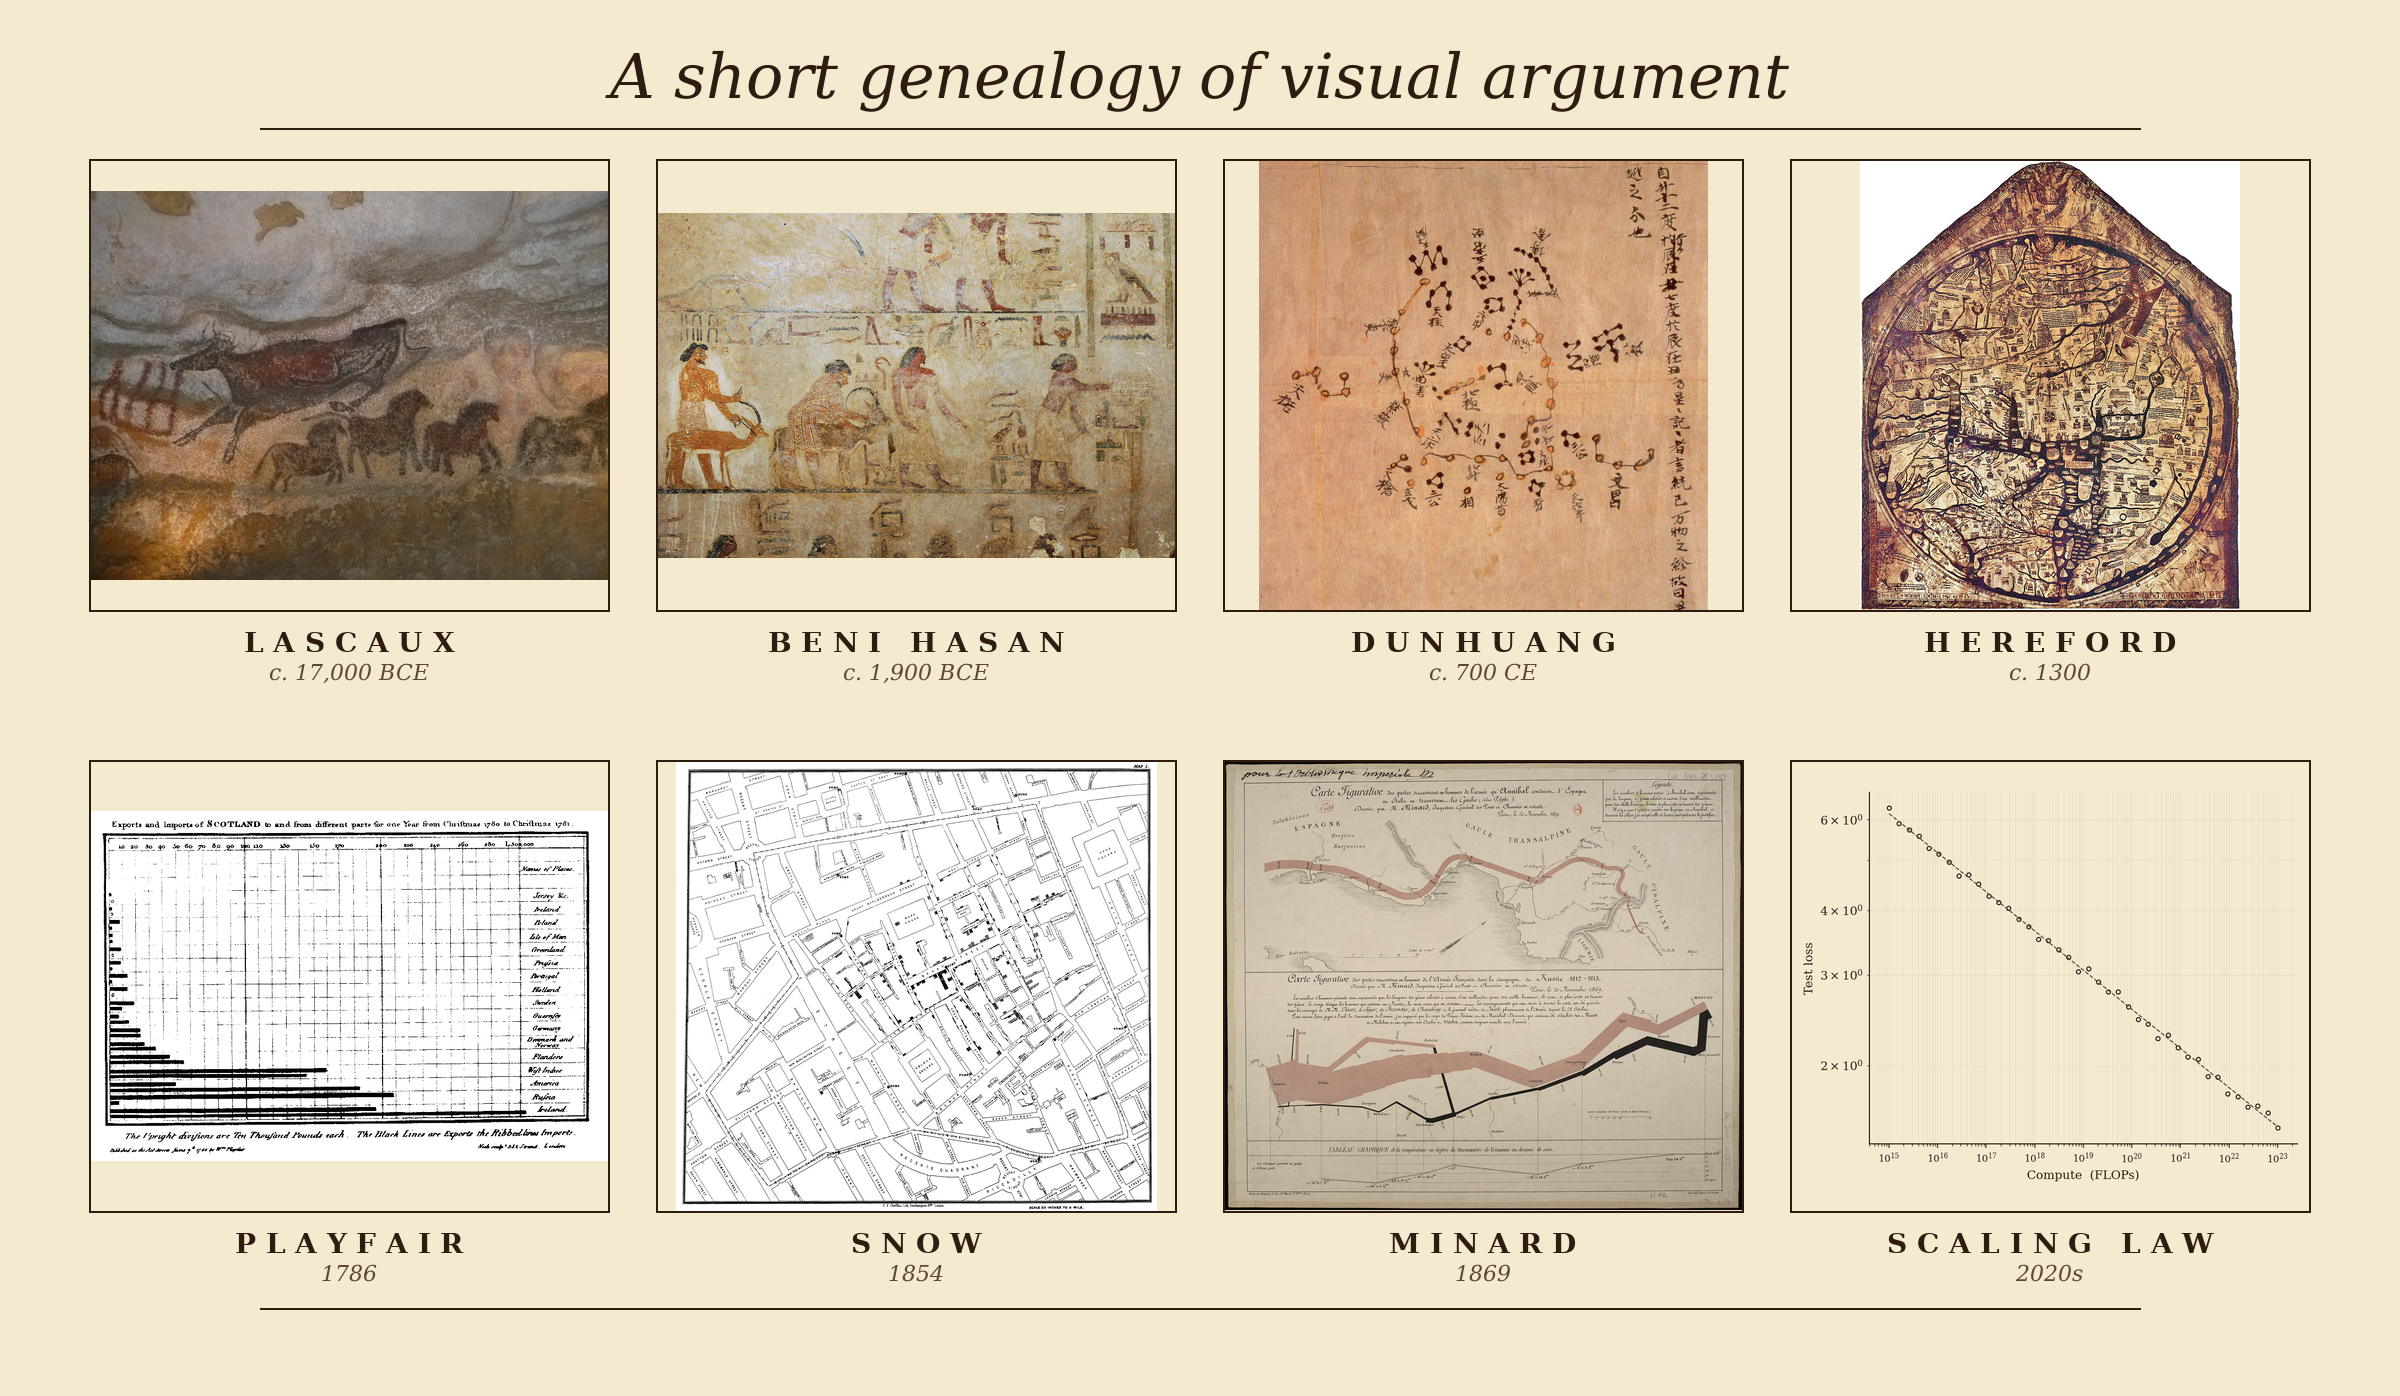
\includegraphics[width=\textwidth]{figures/fig_1_0_evolution.png}
    \caption{}
    \label{fig:visuals-evolution}
  \end{subfigure}

  \vspace{0.4em}

  \begin{subfigure}[t]{\textwidth}
    \centering
    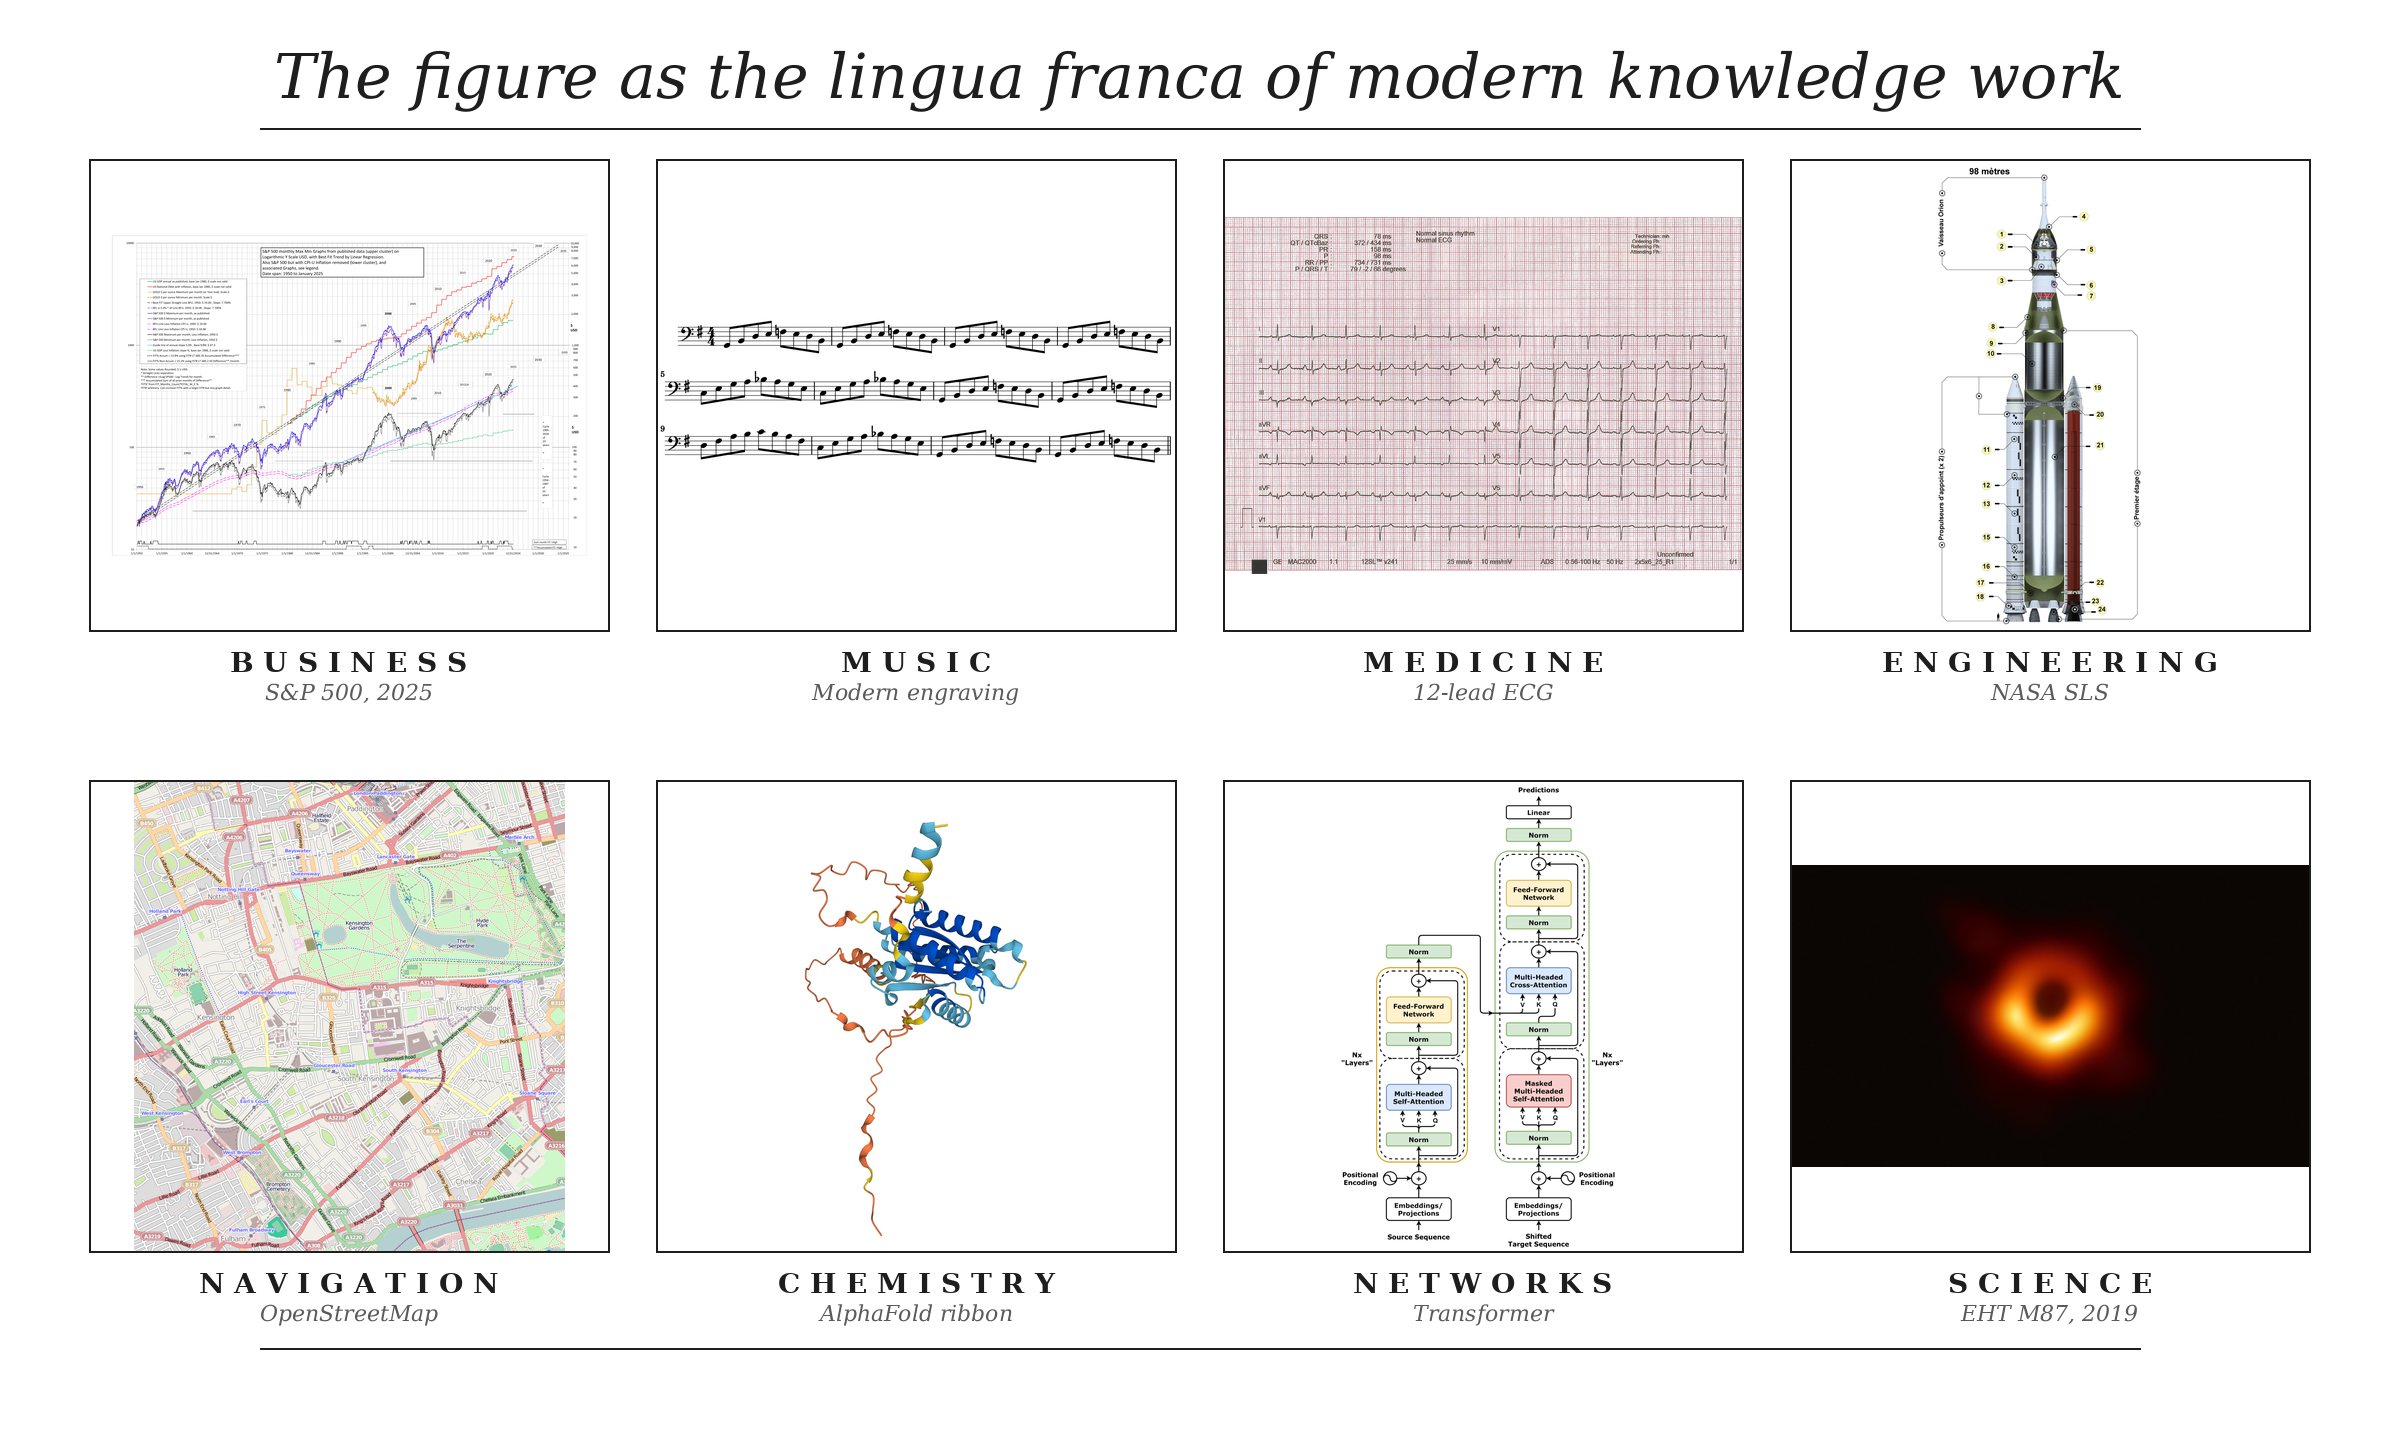
\includegraphics[width=\textwidth]{figures/fig_1_1_fields.png}
    \caption{}
    \label{fig:visuals-fields}
  \end{subfigure}
  \caption[Visual argument, then and now]{\textbf{(a)}~A short
  genealogy of visual argument, from Lascaux and Egyptian wall
  painting through the medieval \emph{mappa mundi}, Playfair's 1786
  bar chart and Snow's 1854 cholera map to modern neural scaling
  curves. \textbf{(b)}~The figure as a lingua franca of modern
  knowledge work across business, music, medicine, engineering,
  navigation, chemistry, networks and the natural sciences.
  {\footnotesize\emph{Sources.} \textbf{(a)}~Lascaux aurochs, Beni
  Hasan caravan, Dunhuang star chart, Hereford \emph{mappa mundi},
  Playfair 1786 bar chart, Snow 1854 cholera map and Minard 1869
  flow map of Napoleon's Russian campaign, all public domain (via
  Wikimedia Commons, the Metropolitan Museum of Art, the British
  Library, Hereford Cathedral, the Internet Archive and the
  Biblioth\`{e}que nationale de France respectively); scaling
  curves adapted from \citealt{kaplan2020scaling}. \textbf{(b)}~A
  candlestick chart, score excerpt, ECG trace, blueprint, nautical
  chart, molecular diagram, network graph and scientific plot,
  from public-domain or openly-licensed repositories (Wikimedia
  Commons, NOAA, PhysioNet) or rendered by the author.}}
  \label{fig:visuals}
\end{figure}

\section{Can \emph{Intelligentia Machinae} (Machine Intelligence) Comprehend Visuals Similarly?}
\label{sec:intro-ai}

Recent progress in artificial intelligence has rapidly normalised
the idea that these systems can be integrated into nearly every
part of working life. Having established that \emph{the human}
is a visual thinker and that \emph{the figure} is a lingua franca
of modern
knowledge work, it becomes imperative to investigate how well the
current frontier of artificial intelligence, in particular the
vision-language models given their present dominance, can navigate the
visual paradigm, since in collaborative work with humans they
will more often than not encounter images.

There is evidence that the best models of today still fail in
some way. Figure~\ref{fig:hero} reproduces a sunburst drawn
from an arXiv paper in the \textsc{SciFig-Eval} corpus. In the original image
the outer-ring category between \emph{Movie Characters} and
\emph{Novel Characters} is legibly \emph{Teleplay Characters}; in
the degraded variant, that single label has been selectively
blurred. Asked which category sits between the two, GPT-5.2,
arguably the most widely used frontier model at the time of
writing, replies ``\emph{Anime Characters}'' and offers no
acknowledgement that the relevant region is unreadable.

\begin{figure}[!ht]
  \centering
  \begin{tikzpicture}
    \node[inner sep=8pt, draw=gray!65, line width=0.6pt,
          fill=white,
          path picture={%
            \draw[step=0.35cm, gray!15, line width=0.2pt]
              (path picture bounding box.south west)
              grid (path picture bounding box.north east);
          }] {%
      \begin{minipage}{0.93\textwidth}
        \centering
        \begin{subfigure}[t]{0.47\linewidth}
          \centering
          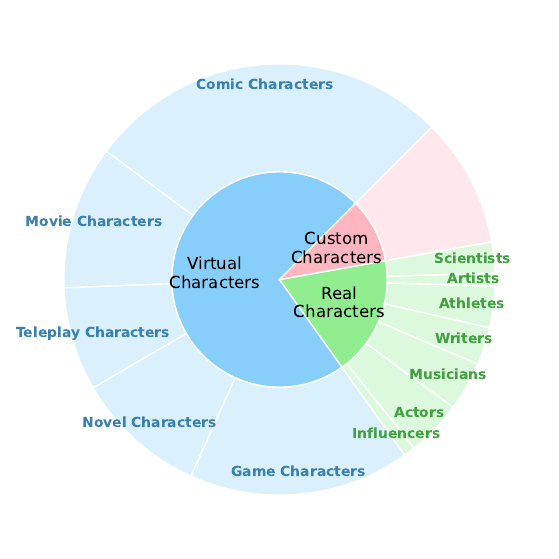
\includegraphics[width=\linewidth]{figures/hero/multi_fig_004_original.png}
          \caption{Original figure.}
          \label{fig:hero-original}
        \end{subfigure}\hfill
        \begin{subfigure}[t]{0.47\linewidth}
          \centering
          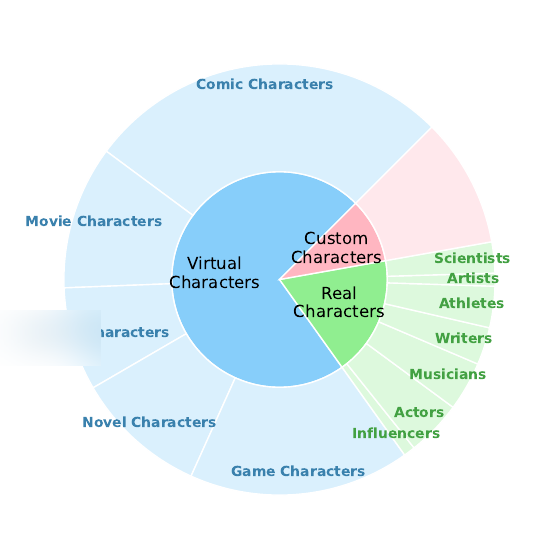
\includegraphics[width=\linewidth]{figures/hero/multi_fig_004_blur.png}
          \caption{One outer label selectively blurred.}
          \label{fig:hero-blur}
        \end{subfigure}
      \end{minipage}%
    };
  \end{tikzpicture}
  \caption[Confabulation under selective blur]{A sunburst from an
  arXiv paper in the \textsc{SciFig-Eval} corpus. In
  \textbf{(a)}, the outer-ring category between \emph{Movie
  Characters} and \emph{Novel Characters} is legibly
  \emph{Teleplay Characters}; in \textbf{(b)}, that single label
  has been blurred. Asked which category sits between the two,
  GPT-5.2 answers ``\emph{Anime Characters},'' with no admission
  that the relevant region is unreadable. Source image reproduced
  from arXiv:2505.23923v1 under its open-access licence; blurred
  variant generated by the \textsc{SciFig-Eval} pipeline.}
  \label{fig:hero}
\end{figure}

Beyond cataloguing such gaps in today's VLMs, it is essential to
understand their behavioural dynamics under a range of visual
stressors and, more importantly, to provide a standardised way
of reading those dynamics from their outputs, so that the
resulting picture can be used to improve the models' capacity to
act as reliable allies in everyday visual work.

\FloatBarrier
\section{Motivation for Focusing on Scientific Research Figures}
\label{sec:intro-research}

Among the domains in which collaborative intelligence is now
being tested at scale, scientific research has moved fastest.
Between late 2024 and early 2026 the three largest model
developers each shipped an autonomous research agent
\citep{google2024gemini_deepresearch, openai2025deepresearch,
anthropic2025research}, and scientific deployments such as the
Biomni biomedical platform now report research-cycle
compressions of an order of magnitude or more
\citep{anthropic2026science}. Scientific argument is also
overwhelmingly visual: every competent empirical paper
eventually commits its claim to a figure, so any system that
hopes to act as a credible research partner must read those
figures with the fidelity its human collaborator does. The
scientific figure is therefore the natural object at which to
test whether the current frontier reads visually or only
appears to.

Science, in addition, is not a monolingual record. A
substantial share of the literature is produced in Chinese,
German, Bulgarian and other languages of research, and the
cost of excluding that share, in citation, uptake and
participation, has been documented at length
\citep{amano2023manifold}. The few multilingual figure-
understanding evaluations now appearing already report
substantial cross-lingual degradation on tasks the same models
solve comfortably in English
\citep{li2025polychart, gao2025pm4bench, sharma2025indicvision},
which is to say that a figure-reader reliable only in English
is, as a research collaborator, structurally partial. The
scientific figure considered across languages, then, is what
the present work takes as its test object.

\section{Research Questions}
\label{sec:intro-rqs}

The central objective of this thesis is to characterise, across
models, languages and adversarial conditions, how faithfully
today's frontier multimodal models actually read scientific
figures, and to build an evaluation framework that surfaces the
failure modes which conventional accuracy benchmarks obscure.
Concretely, the investigation is organised around the following
four research questions, each pairing a capacity with the
conditions under which that capacity is tested:

\begin{description}
\item[RQ1 (Faithful figure description across languages).] To what
  extent do current vision--language models produce accurate,
  complete and clearly expressed descriptions of scientific figures
  across typologically diverse languages?

\item[RQ2 (Robustness to visual degradation).] How does visual
  degradation, including noise, compression, aspect distortion and
  contextual embedding within paper pages, affect the accuracy
  (whether what is stated is correct), completeness (whether what
  is visible is reported) and clarity (whether what is reported is
  expressed unambiguously) of VLM-generated figure descriptions?

\item[RQ3 (Comprehension beyond description).] Beyond surface
  description, can VLMs demonstrate genuine comprehension of
  scientific visualisations, from answering quantitative
  questions to performing non-trivial inductive reasoning that
  requires distinguishing analytical insight from surface-level
  pattern matching?

\item[RQ4 (Behavioural dynamics under stress).] How do VLMs
  behave when the visual evidence or its accompanying context
  is stressed, for example through misleading captions,
  contradictory premises, sycophancy probes, or images whose
  answer is no longer pixel-recoverable? In particular, do
  they hold a faithful reading of the figure, adopt the
  position the prompt implies, or acknowledge that the
  available evidence does not support a confident answer?
\end{description}

\section{Research Contributions}
\label{sec:intro-contributions}

In addressing these questions, the thesis makes three contributions.

\begin{description}
\item[C1: \textsc{SciFig-Eval}, a multilingual benchmark for
  scientific figure understanding.] We release a corpus of 1{,}005
  figures from 349 papers across native-language venues, paired with 1{,}411 expert
  annotations in English, Bulgarian, German and Chinese, and
  augmented by a 45-figure adversarial subset covering nine image
  transforms. Figure understanding is scored along three
  MQM-adapted axes --- accuracy, completeness and clarity ---
  through a dual-judge pipeline designed to control for known
  judge-model biases.

\item[C2: A psychology-informed adversarial probe design.] Grounded
  in the misinformation effect and the anchoring bias from cognitive
  psychology, we construct four probe families --- hallucination,
  caption-bias, visual degradation, and prompt-reversal ---
  that target distinct stages of the VLM pipeline, from the visual
  encoder through cross-modal alignment to the autoregressive
  decoder, and expose failure modes that conventional accuracy
  benchmarks conflate.

\item[C3: The Admittance--Resistance--Inductance behavioural
  framework.] We propose a three-axis behavioural framework,
  inspired by the electrical metaphor, that decomposes figure-reading
  trustworthiness into \emph{Admittance} (honesty in the absence of
  evidence), \emph{Resistance} (faithfulness under misleading
  context) and \emph{Inductance} (sound inductive reasoning).
  Applied across thirteen contemporary models from six families, the
  three axes capture distinct failure modes, recasting trustworthiness as a
  behavioural profile rather than a single scalar.
\end{description}

\section{Thesis Structure}
\label{sec:intro-structure}

The remainder of the thesis is organised as follows.
Chapter~2 (Background) provides the technical and conceptual
foundation: how frontier multimodal models convert figures into
internal representations, how scientific figures carry argument
rather than merely depict it, and the failure modes and evaluation
traditions on which the remainder draws.
Chapter~3 (Literature Survey) situates the work against chart
understanding, multimodal hallucination, multilingual evaluation
and MQM-style scoring.
Chapter~4 (Design) sets out the SciFig corpus, the A--R--I
framework and the four adversarial probe families.
Chapter~5 (Implementation) describes the evaluation pipeline, the
model and judge harness and the reproducibility controls.
Chapter~6 (Evaluation) reports the main quantitative results
across the 13 evaluated models and the four languages, together
with ablations on judge ensembles and probe families.
Chapter~7 (Discussion) interprets the findings, connects them to
the A--R--I framework and acknowledges the limitations of the
study.
Chapter~8 (Conclusion) summarises the contributions, revisits the
research questions and outlines directions for future work.

The full source code, evaluation scripts and reproducibility controls are publicly available at \url{https://github.com/WeNLP4Science-Lab/SciFig-Evaluation}.
An interactive visualisation dashboard for exploring per-figure, per-model and per-language results is deployed at \url{https://victorious-glacier-00483810f.2.azurestaticapps.net}.
